\documentclass[10pt,a4paper]{article}
\usepackage[utf8]{inputenc}
\usepackage[T1]{fontenc}
\usepackage{charter}
\usepackage{geometry}
\geometry{a4paper, margin=18mm}
\usepackage{graphicx}
\usepackage{tikz}
\usepackage{hyperref}
\hypersetup{colorlinks=true, linkcolor=black, urlcolor=black}

\pagestyle{empty}
\linespread{1.08}

\newcommand{\iconEnvelope}{%

\begin{tikzpicture}[x=0.075em, y=0.075em, baseline=-0.22em]
  \draw[line width=0.55pt, rounded corners=0.4pt, fill=black] (0,0) rectangle (12,8.2);
  \draw[line width=0.5pt, color=white] (0.8,7.5) -- (6,3.5) -- (11.2,7.5);
\end{tikzpicture}%
}
\newcommand{\iconPhone}{%

\begin{tikzpicture}[x=0.065em, y=0.065em, baseline=-0.22em]
  \draw[line width=1.0pt, line cap=round, line join=round, fill=black] 
    (2,8.5) .. controls (1.5,9.5) and (3,10.5) .. (4.2,10.2)
    -- (5.3,8.5) .. controls (5.6,8) and (5.2,7.3) .. (4.6,7.1)
    -- (4.1,7) .. controls (4.4,5.4) and (5.4,4.4) .. (7,4.1)
    -- (7.1,4.6) .. controls (7.3,5.2) and (8,5.6) .. (8.5,5.3)
    -- (10.2,4.2) .. controls (10.5,3) and (9.5,1.5) .. (8.5,2)
    .. controls (5,2) and (2,5) .. (2,8.5) -- cycle;
\end{tikzpicture}%
}
\newcommand{\iconLocation}{%

\begin{tikzpicture}[x=0.075em, y=0.075em, baseline=-0.22em]
  \path[fill=black] (5,10) .. controls (2.2,10) and (0,7.8) .. (0,5)
    .. controls (0,1.8) and (5,-2) .. (5,-2)
    .. controls (5,-2) and (10,1.8) .. (10,5)
    .. controls (10,7.8) and (7.8,10) .. (5,10) -- cycle;
  \fill[white] (5,5.2) circle (1.8);
\end{tikzpicture}%
}

\begin{document}

\begin{center}
  {\fontsize{22}{26}\selectfont \textbf{THÉODORE HESLING}}\\[4pt]
  {\fontsize{11}{13}\selectfont \textit{Élève-Ingénieur Mines Saint-Étienne (ISMIN) -- Recherche de Stage Suisse 2027}}\\[5pt]
  {\fontsize{8.5}{10.5}\selectfont 
    \iconEnvelope~theodore200531@outlook.com \quad
    \iconPhone~+33 6 75 49 33 72 \quad
    \iconLocation~Gardanne 13120, France
  }\\[7pt]
  \rule{\textwidth}{0.8pt}
\end{center}

\vspace{6pt}

\begin{center}
  {\Large \textbf{Fiche Récapitulative des QR Codes de Candidature}}\\[4pt]
  {\small Flashez un QR code avec l'appareil photo de votre smartphone pour accéder directement au profil ou au CV.}
\end{center}

\vspace{18pt}

% ROW 1: LINKEDIN & CV 1
\noindent
\begin{minipage}[t]{0.48\textwidth}
  \centering
  {\large \textbf{Profil LinkedIn}}\\[6pt]
  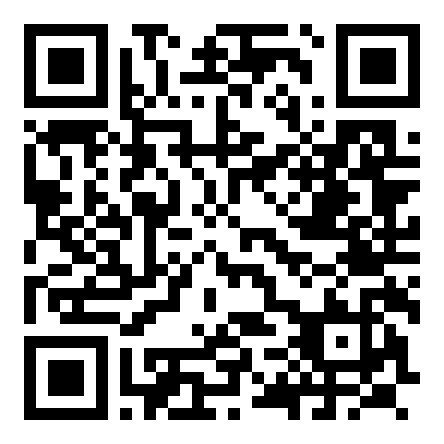
\includegraphics[width=42mm]{qrcode_linkedin.png}\\[6pt]
  {\textbf{Théodore Hesling}}\\[2pt]
  {\footnotesize Réseau, recommandations et parcours complet}\\[2pt]
  {\scriptsize \href{https://www.linkedin.com/in/th%C3%A9odore-hesling-a08316386}{\texttt{linkedin.com/in/théodore-hesling-a08316386}}}
\end{minipage}\hfill
\begin{minipage}[t]{0.48\textwidth}
  \centering
  {\large \textbf{CV 1 : Systèmes Embarqués}}\\[6pt]
  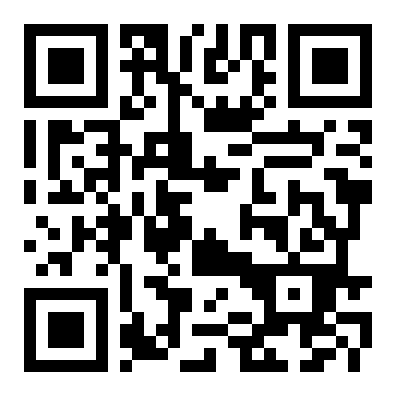
\includegraphics[width=42mm]{qrcode_cv1_embedded_security.png}\\[6pt]
  {\textbf{Embedded \& Hardware Security}}\\[2pt]
  {\footnotesize STM32 bare-metal, Cryptographie, Secure Boot}\\[2pt]
  {\scriptsize \href{https://hesgacreation.github.io/cv/cv1.pdf}{\texttt{hesgacreation.github.io/cv/cv1.pdf}}}
\end{minipage}

\vspace{26pt}

% ROW 2: CV 2 & CV 3
\noindent
\begin{minipage}[t]{0.48\textwidth}
  \centering
  {\large \textbf{CV 2 : Cybersécurité \& Infra}}\\[6pt]
  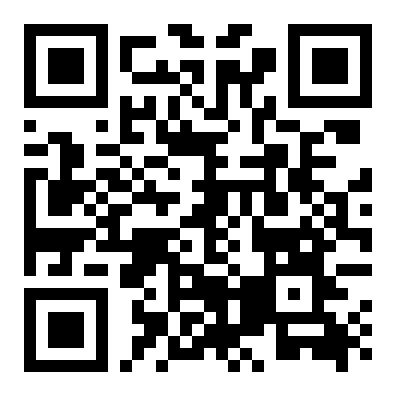
\includegraphics[width=42mm]{qrcode_cv2_cybersecurity_infra.png}\\[6pt]
  {\textbf{Cybersecurity \& Infrastructure}}\\[2pt]
  {\footnotesize OpenSSL, Réseaux, Hardening Linux, Détection}\\[2pt]
  {\scriptsize \href{https://hesgacreation.github.io/cv/cv2.pdf}{\texttt{hesgacreation.github.io/cv/cv2.pdf}}}
\end{minipage}\hfill
\begin{minipage}[t]{0.48\textwidth}
  \centering
  {\large \textbf{CV 3 : Robotique \& Capteurs}}\\[6pt]
  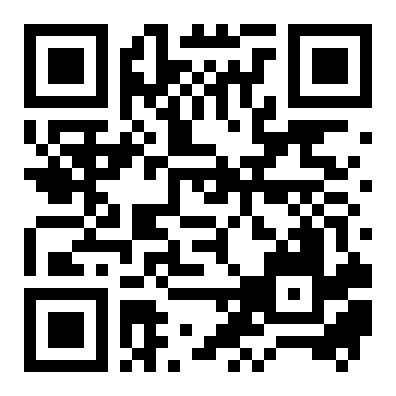
\includegraphics[width=42mm]{qrcode_cv3_robotics_sensors.png}\\[6pt]
  {\textbf{Robotics, Sensors \& Autonomy}}\\[2pt]
  {\footnotesize Capteurs capacitifs différentiels, PID, CAO Inventor}\\[2pt]
  {\scriptsize \href{https://hesgacreation.github.io/cv/cv3.pdf}{\texttt{hesgacreation.github.io/cv/cv3.pdf}}}
\end{minipage}

\vfill
\begin{center}
  \rule{0.6\textwidth}{0.4pt}\\[6pt]
  {\footnotesize \textbf{Mobilité Suisse :} Citoyen français (UE) -- Éligible aux permis suisses B/L simplifiés sans quota.\\
  Disponible à partir d'avril 2027 pour un stage de 4 à 5 mois (validation quitus CTI 16 semaines).}
\end{center}

\end{document}
